\subsection{Open Loop Time Response}\label{s:time_response}

Now that the solutions to the first and second order systems have been derived using both the characteristic and particular solution method as well as the Laplace transform method, the time response of these systems can be analyzed. The time response of a system is the output of the system as a function of time given a specific input. The time response can be used to analyze the stability and performance of the system. 

\subsubsection{Position and Velocity Response of a Car}

First, let's plot the time response of the first order system given by equation \ref{e:first_order_solution} as well as the second order solution given by equation \ref{e:position_car_solution}. The parameters for the system are chosen to be $F_0=1000~N$, $c=50~Ns/m$, and $m=1000~kg$. The initial velocity and position are assumed to be zero. In order to show the time response however, 3 different curves will be placed on the graph. The first will be the analytic solution to the first and second order system, the second is the Laplace transform solution using the control systems toolbox in Python and the last is the numerical integration of the equations of motion. The python code used to generate this is shown in the Figure below and also available on \href{https://github.com/cmontalvo251/Python/blob/master/controls/first_order_system.py}{GitHub}.
\begin{figure}[H]
\centering
\begin{minipage}{0.48\textwidth}
\centering
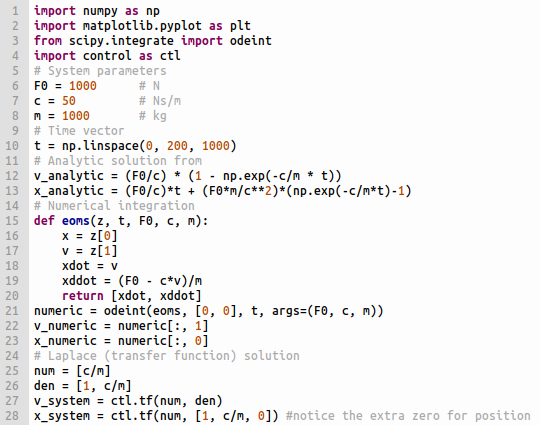
\includegraphics[width=\linewidth]{Figures/car_code_1.png}
\end{minipage}\hfill
\begin{minipage}{0.48\textwidth}
\centering
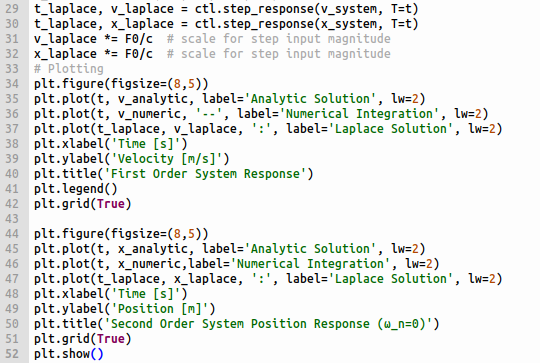
\includegraphics[width=\linewidth]{Figures/car_code_2.png}
\end{minipage}
\caption{Python code to generate the time response of a car}
\label{f:car_code}
\end{figure}
Note the code is commented to help the reader understand what is happening. Note the benefit of using the control systems toolbox in Python. The time response can be generated by first creating the transfer function and then applying a step to the transfer function. This will come in handy later when it is necessary to apply a control system to the transfer function before inversing back to the time domain. The numerical integration is also useful when the equations of motion are known and the control system designer wants to work in the time doman rather than the laplace domain. It's also very helpful when the system is non-linear since transfer functions only work for linear systems. All three methods have their pros and cons. The numerical integration is done using the scipy.integrate.odeint function which is a simple way to numerically integrate ordinary differential equations. The results of the time response are shown in Figure \ref{f:car_response}.
\begin{figure}[H]
\centering
\begin{minipage}{0.48\textwidth}
\centering
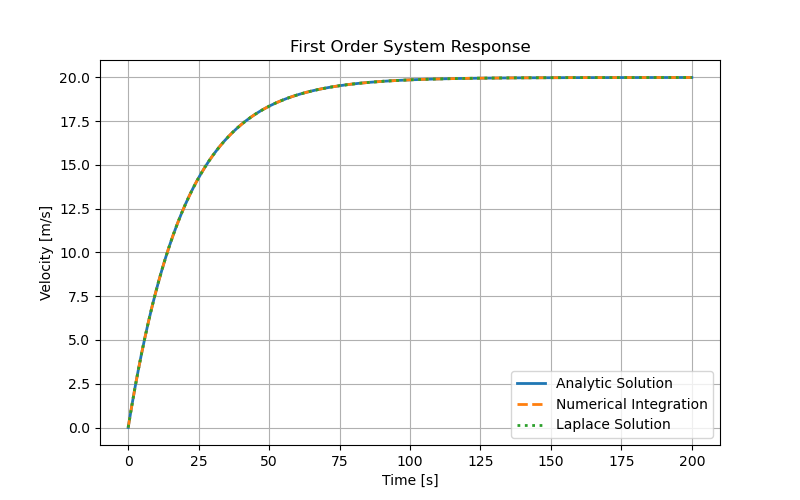
\includegraphics[width=\linewidth]{Figures/car_velocity_response.png}
\end{minipage}\hfill
\begin{minipage}{0.48\textwidth}
\centering
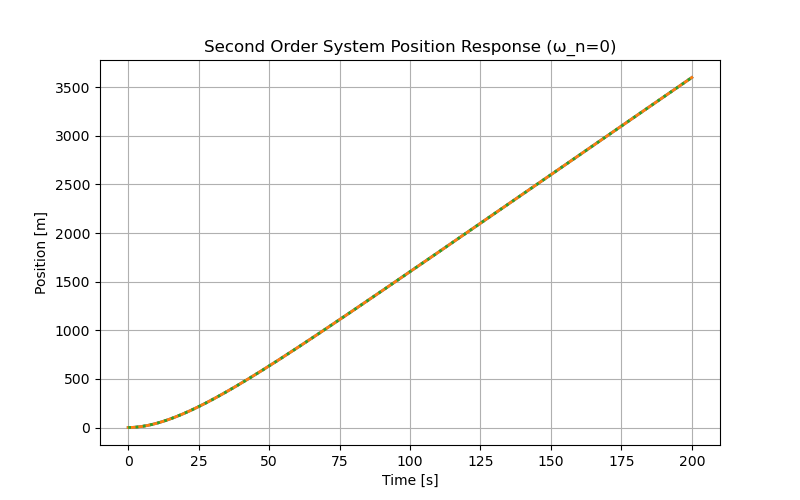
\includegraphics[width=\linewidth]{Figures/car_position_response.png}
\end{minipage}
\caption{Time response of the position (right) and velocity (left) of a car}
\label{f:car_response}
\end{figure}
\noindent The time response shows that the velocity of the car asymptotically approaches a steady state value of $F_0/c = 20~m/s$. The time constant of the system is $\tau = m/c = 20~s$. The time constant is the time it takes for the system to reach 63.2\% of its steady state value. The settling time $T_s=4\tau$ is the time the system takes to get within 2\% of its final value. In this case that is $80~s$. The time response can be used to analyze the stability and performance of the system. In this case, the system is stable and the performance is acceptable given the parameters chosen. However, examining the position of the car shows that the position will continue to increase linearly over time. This is because the car is moving at a constant velocity. The position of the car will not reach a steady state value but rather continue to increase linearly over time. This is an example of a marginally stable system. The velocity of the car is stable while the position of the car is marginally stable.

\subsubsection{Position of a Mass Spring Damper}

Simulating the mass spring damper is very similar to the car example. The parameters for the system are chosen to be $F_0=1000~N$, $k=2000~N/m$, $c=50~Ns/m$, and $m=100~kg$. The initial position and velocity are assumed to be zero. The python code used to generate this is shown in the Figure below and also available on \href{https://github.com/cmontalvo251/Python/blob/master/controls/mass_spring_damper.py}{GitHub}. 
\begin{figure}[H]
\centering
\begin{minipage}{0.48\textwidth}
\centering
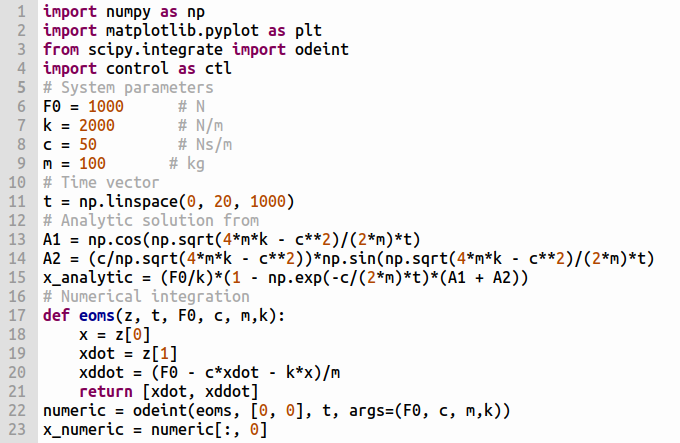
\includegraphics[width=\linewidth]{Figures/mass_spring_damper_code_1.png}
\end{minipage}\hfill
\begin{minipage}{0.48\textwidth}
\centering
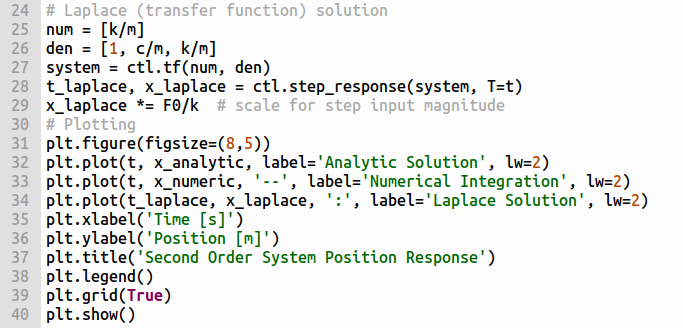
\includegraphics[width=\linewidth]{Figures/mass_spring_damper_code_2.png}
\end{minipage}
\caption{Python code to generate the time response of a mass spring damper}
\label{f:mass_spring_damper_code}
\end{figure}
Note the code is commented to help the reader understand what is happening. Again, the simulation is run by integrating the equations of motion, applying a step response to the transfer function and also plotting the analytic solution. The results of the time response are shown in Figure \ref{f:mass_spring_damper_response}.
\begin{figure}[H]
\centering
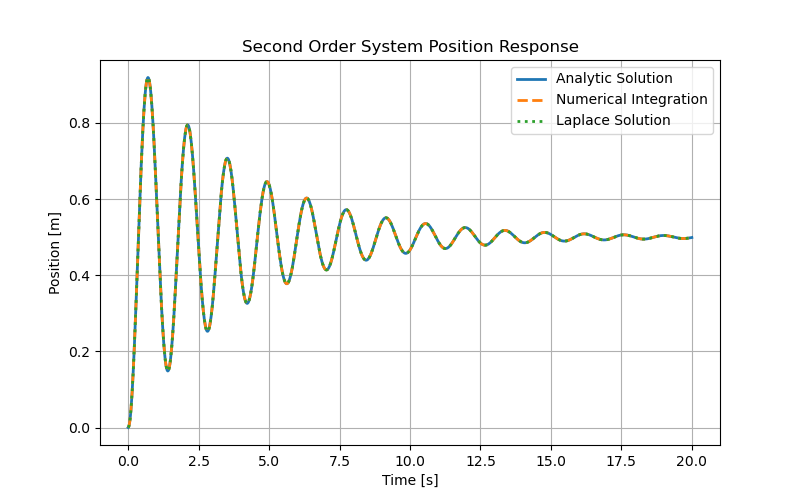
\includegraphics[width=0.8\linewidth]{Figures/mass_spring_damper_response.png}
\caption{Time response of the position of a mass spring damper}
\label{f:mass_spring_damper_response}
\end{figure}
\noindent The time response shows that the position of the mass spring damper reaches a steady state value of $F_0/k = 0.5~m$. The time constant of the system is $\tau = 2m/c = 4~s$. The natural frequency of the system is $\omega_n = \sqrt{k/m} = 4.47~rad/s$. The damping ratio of the system is $\zeta = c/(2 m\omega_n) = 0.056 (underdamped)$. The settling time $T_s=4/(\zeta \omega_n)$ is the time the system takes to get within 2\% of its final value. In this case that is $16~s$. Notice that $T_s=4\tau$ where again $\tau = 4~s$. The time response can be used to analyze the stability and performance of the system. In this case, the system is stable and the performance is acceptable given the parameters chosen. Here are some useful equations for natural frequency, settling time and other second order parameters.
\begin{equation}
    \begin{matrix}
    \omega_n = \sqrt{\frac{k}{m}} & T_s = \frac{4}{\zeta \omega_n} & \tau = \frac{2m}{c} \\
    \zeta = \frac{c}{2m\omega_n} & \omega_d = \omega_n \sqrt{1-\zeta^2} & T_s = 4\tau \\
    \omega_n = 2\pi f & f = \frac{1}{T} & \tau = \frac{1}{\zeta \omega_n} 
    \end{matrix}
\end{equation}

\subsubsection{Attitude of a Satellite or Quadcopter}

Recall for the satellite/quadcopter example the equation of motion was given as $\ddot{\theta} = \frac{2F d}{J}$ and the transfer function was given as $\frac{\Theta(s)}{F(s)}= G(s) = \frac{2d}{Js^2}$. The solution to this system due to a step function was shown in the general solution to second order systems with the special case that the natural frequency and damping ratio was zero. The solution then given as $\theta(t) = \frac{F_0 d}{J} t^2$ which increases quadratically over time. The python code used to generate this is also available on \href{https://github.com/cmontalvo251/Python/blob/master/controls/satellite.py}{Github}. The code is not shown here as it is very similar to the previous two examples. Again the code is commented to help the reader understand what is happening. The simulation is run by integrating the equations of motion, applying a step response to the transfer function and also plotting the analytic solution. The results of the time response are shown in Figure \ref{f:satellite_response}. For this specific case $F_0=0.1~N$ , $d=0.5~m$ and $J=10~kg-m^2$.
\begin{figure}[H]
\centering
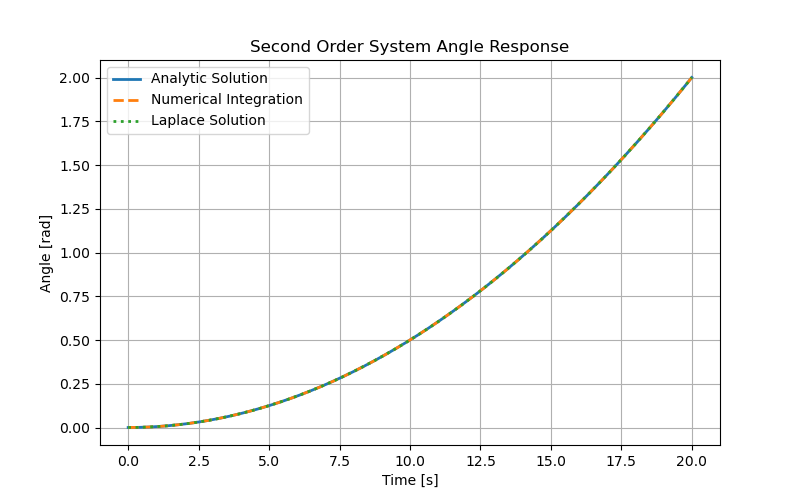
\includegraphics[width=0.8\linewidth]{Figures/satellite_response.png}
\caption{Time response of the attitude of a satellite/quadcopter}
\label{f:satellite_response}
\end{figure}
\noindent The time response shows that the attitude of the satellite/quadcopter increases quadratically over time. This is because there is no restoring moment or damping moment acting on the system. The system is marginally stable as the attitude will continue to increase over time and this will be discussed in more detail in section \ref{s:stability}.

\subsubsection{Pitch Response of an Aircraft}\label{s:aircraft_pitch_response}

The solution for the pitch response of an aircraft is very similar response to the mass spring damper system given the second order nature of the system. The difference lies in the natural frequency and damping ratio. For the mass spring damper example the system oscillated quite a bit with a damping ratio of $\zeta = 0.056$ which is quite underdamped. As such, many oscillations were present. For the case of the attitude dynamics of an aircraft the "short period" mode of the aircraft is quite quick and highly damped as will be shown below. Note that a standard aircraf has 5 general mode shapes due to the six degree of freedom nature of the aircraft. However, for this simple 2-D analysis of pure pitch motion about the center of mass, only the "short period" mode is seen. This mode is due to the lift generated by the tail and the stability derivative $C_{mq}$. In order to simulate this second order system an example aircraft must be used. The aircraft utilized for this analysis is an E-flite Apprentice S15e airplane \cite{apprentice} as shown in Figure \ref{f:apprentice}. This aircraft is a three wheeled high wing trainer made of a patented Z-Foam that allows the airplane to be durable yet lightweight. The wing has a constant Clark-Y airfoil with a chord length of 0.75 ft. The wingspan of the aircraft is 4.92 ft. Using a fish scale, the total weight of each aircraft was found to be 2.72 lbf ($0.0844 slugs$). Inertia estimates were crude rectangular prism estimates assuming even distribution of mass The inertias were found to be $I_{xx} = 0.17,I_{yy} = 0.09,I_{zz} = 0.25~slugs-ft^2$. The airplane is equipped with an 840 kV brushless outrunner motor, 30-Amp pro switch-mode BEC brushless ESCs, three digital micro servos to control the aileron and the elevator, and a larger standard servo that controls the rudder and the front wheel of the landing gear. The aircraft is equipped with a 3000 mAh 3S LiPo battery and a trim velocity of $65.6 ft/s (20~m/s)$.
\begin{figure}[H]
\centering
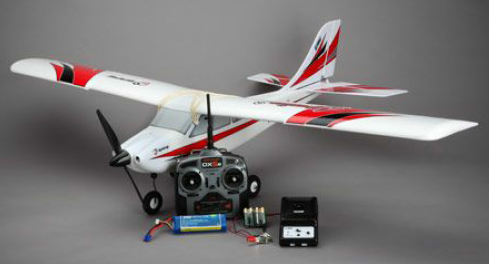
\includegraphics[width=0.6\linewidth]{Figures/apprentice.PNG}
\caption{Apprentice S 15e Aircraft}
\label{f:apprentice}
\end{figure}
This aircraft has been used by the (Faciliy for Aerospace Systems and Technology) \href{http://www.aerialsystems.org/}{FAST Lab} for many flight tests. While the mass and geomtric parameters have been explained above, the aerodynamic coefficients have been reported in many sources \cite{Cobar_FASTSim_AVIATION_2022,CobarMeta2019,CobarMASTERS}. The aerodynamic coefficients from a previous state estimation report are given in the Table below\cite{CobarMeta2019}.
\begin{table}[H]
\begin{center}
\caption{Estimated Aerodynamic Coefficients after System
  Identification Procedure}
\begin{tabular}{cccccccccccc}
  \hline
  $C_{L_{0}}$ & $C_{D_{0}}$ & $C_{m_{0}}$ & $C_{L_{q}}$ & $C_{m_{q}}$  & $C_{L_{\alpha}}$ & $C_{D_{\alpha}}$ & $C_{m_{\alpha}}$ &  $C_{L_{{\delta}e}}$  & $C_{m_{{\delta}e}}$ & $C_{y_{{\delta}r}}$ &  $C_{y_{\beta}}$ \\
  0.34       & 0.017     & { -0.076}       &  5.94       &
    -24.45 &  5.19  &  1.01         & { -2.19}        & 0.41 &
  {-1.15} &  0.069 &  -0.24 \\
  \hline
  $C_{y_{p}}$ & $C_{y_{r}}$ & $C_{l_{\beta}}$ &  $C_{l_{p}}$ & $C_{l_{r}}$ &   $C_{n_{\beta}}$ &  $C_{n_{p}}$&  $C_{n_r}$ & $C_{l_{{\delta}a}}$ &  $C_{l_{{\delta}r}}$ &  $C_{n_{{\delta}a}}$ & $C_{n_{{\delta}r}}$ \\
  -0.028    & 0.18      &  -0.016       & {-0.50}    &  0.098   &
  { 0.088}
  & { -0.788}      &  {-0.069}          &  { 0.28} & 0.0047
  & { 0.06} & { -0.17}\\
  \hline
\end{tabular}
\label{t:aerofinal}
\end{center}
\end{table}
\noindent Using these coefficients, the mass and geometry properties, similar code can be used to plot the time response of the system. As dicussed previously, the equations of motion of the pitch dynamics of an aircraft are given as 
\begin{equation}
    \ddot{\theta} + \left(-\frac{\rho V^2 S \bar{c}^2 C_{mq}}{4I_{yy} V}\right)\dot{\theta} + \left(-\frac{\rho V^2 S \bar{c} C_{m\alpha}}{2I_{yy}}\right)\theta = -\frac{\rho V^2 S \bar{c} C_{m\delta_e}}{2I_{yy}}\delta_e
\end{equation}
To find the transfer function, a few substitutions are made to simplify the equation. Let
\begin{equation}
    \begin{matrix}
    \lambda_1 = -\frac{\rho V^2 S \bar{c}^2 C_{mq}}{4I_{yy} V} &
    \lambda_2 = -\frac{\rho V^2 S \bar{c} C_{m\alpha}}{2I_{yy}} &
    \kappa = -\frac{\rho V^2 S \bar{c} C_{m\delta_e}}{2I_{yy}}
\end{matrix}
\end{equation}
The equation of motion can then be rewritten as
\begin{equation}
    \ddot{\theta} + \lambda_1 \dot{\theta} + \lambda_2 \theta = \kappa \delta_e
\end{equation}
Taking the laplace transform of both sides and assuming zero initial conditions gives
\begin{equation}
    \frac{\Theta(s)}{\Delta_e(s)} = G(s) = \frac{\kappa}{s^2 + \lambda_1 s + \lambda_2}
\end{equation}
Using the equations of motion as well as the general solution for a second order system the time response itself can be put here. Note that for a typical aircraft the system is stable given the negative $C_{m\alpha}$. Above notice that $C_{m\alpha}=-2.19$ However, as is the case with the F-16 fighter jet, some aircraft are designed to be slightly unstable in pitch in order to increase maneuverability. In this case $C_{m\alpha}$ is positive rather than negative which makes the natural frequency imaginary and the system unstable. This will be discussed in more detail in section \ref{s:stability}. However, for now the system will be simulated for both a positive and negative $C_{m\alpha}$ to highlight the potential instability in attitude dynamics of an aircraft. The time response of both simulations is shown below. The code used to generate these plots is  on \href{https://github.com/cmontalvo251/Python/blob/master/controls/pitch_dynamics_apprentice.py}{Github}. Also note that $\rho=0.00238~slugs/ft^3$.
\begin{figure}[H]
\centering
\begin{subfigure}[b]{0.48\textwidth}
\centering
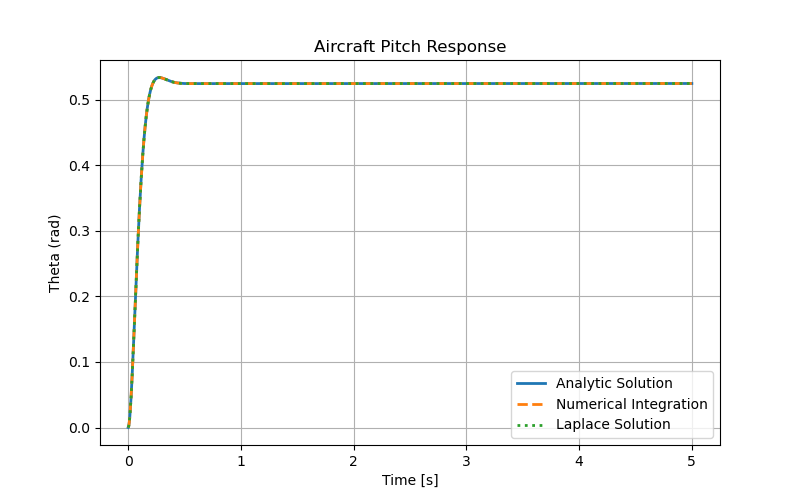
\includegraphics[width=\linewidth]{Figures/aircraft_response_stable.png}
\end{subfigure}
\hfill
\begin{subfigure}[b]{0.48\textwidth}
\centering
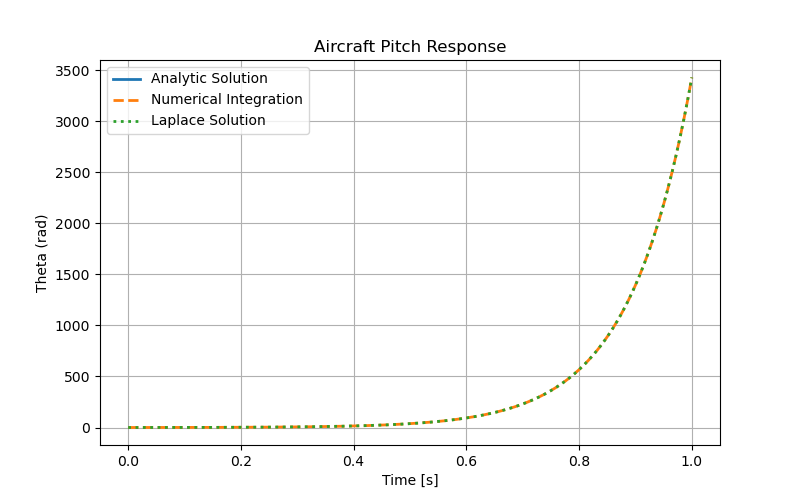
\includegraphics[width=\linewidth]{Figures/aircraft_response_unstable.png}
\end{subfigure}
\caption{Attitude Response of an Aircraft ($C_{m\alpha}=-2.19$ left) ; ($C_{m\alpha}=2.19$ right)}
\label{f:aircraft_response}
\end{figure}
First, examining the plot on the left, the system is indeed second order and oscillates but the oscillations are damped out significantly faster than in the mass spring damper case. This is because $\zeta = 0.79$ which is so much closer to 1. Remember that a system with $\zeta=1$ is a critically damped system. Therefore, this short period aircraft dynamic simulation is a lot closer to being critically damped than it is underdamped. The plot on the right is generated by setting $C_{m\alpha}=2.19$ which is positive causing the aircraft to be statically unstable. This results in the system diverging off to infinity rather than settling to a steady state value. These unstable systems require a sophisticated control system to ensure the system remains stable and doesn't cause the aircraft to spin wildly out of control.

\subsubsection{Pitch Response of a Rocket}\label{s:rocket_response}

The pitch dynamics of a rocket can be formulated in the same second-order framework used for aircraft and the mass-spring-damper example. The difference in this system lies with the assumption that there is no damping. Recall that the equations of motion of the rocket are as follows:
\begin{equation}
    \ddot{\theta} + \lambda \theta = \kappa \beta
\end{equation}
where $\lambda=\frac{\pi}{J8}\rho V^2 d^2 a$ and $\kappa=\frac{Tb}{2J}$. In reality the lack of damping is not necessarily true but the formulation is done just to highlight what would happen if no damping is present in the system. For the system above the transfer function is
\begin{equation}
  \frac{\Theta(s)}{B(s)} = G(s) = \frac{\kappa}{s^2+\lambda}
\end{equation}
The analytic solution is then the same for the second order case assuming that the damping ratio $\zeta=0$. Using similar code to the spring mass damper system the response to a step input can be shown below assuming the rocket is a small hobbyist grade rocket. 
\begin{figure}[H]
\centering
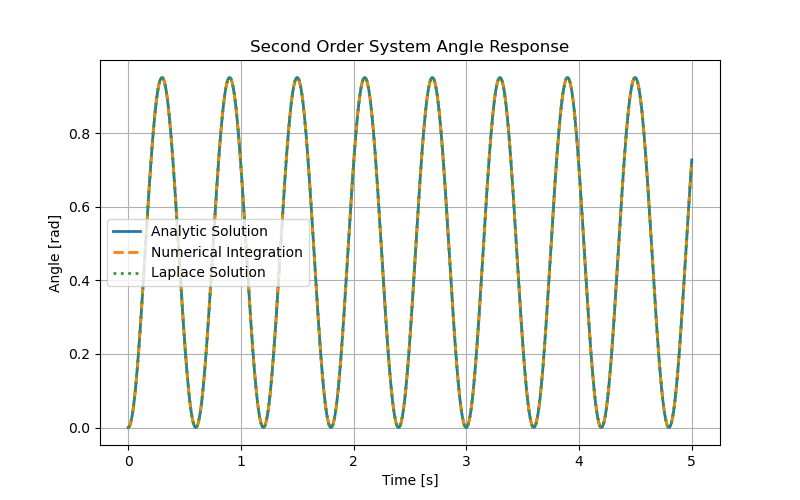
\includegraphics[width=0.8\linewidth]{Figures/rocket_response.png}
\caption{Time response of the attitude of a rocket with TVC}
\label{f:rocket_response}
\end{figure}
\noindent In this simulation above $\rho=0.00238~slugs/ft^3,V=150~ft/s,d=1.0~ft,a=3.0~ft,T=10~lbf,b=6~ft$ and $J=0.57~slugs/ft^3$. The python code used to generate this is on \href{https://github.com/cmontalvo251/Python/blob/master/controls/rocket.py}{GitHub}. The time response shows an interesting result in that the rocket will continue to oscillate forever. Naturally this would be impossible in real life again given the drag created by aerodynamics but for academics sake it is interesting to look at a system that has no damping and oscillates forever. A system like this would be considered marginally stable but of course that will be explained in more detail in section \ref{s:stability}.

\subsubsection{Angle of an Inverted Pendulum}

\hl{Remember since you ran out of your quota for Copilot you can add Gemini back into VS code. The directions are in your personal Gemini and make sure to add it to your VS_Code_Installation_Guide.md}